\documentclass[11pt]{article}

% ---------------------------------------------------------------------------
%  SynLethGNN -- SRI Research Proposal
%  Compile with:  tectonic docs/proposal.tex
% ---------------------------------------------------------------------------

\usepackage[margin=1in]{geometry}
\usepackage{amsmath,amssymb}
\usepackage{xcolor}
\usepackage{tikz}
\usetikzlibrary{arrows.meta,positioning,fit,backgrounds,calc,shapes.geometric,shapes.misc}
\usepackage{booktabs}
\usepackage{array}
\usepackage{colortbl}
\usepackage[most]{tcolorbox}
\usepackage{enumitem}
\usepackage{graphicx}
\usepackage[colorlinks=true,linkcolor=sriblue,citecolor=sriblue,urlcolor=sriaccent]{hyperref}

% ----- Palette -------------------------------------------------------------
\definecolor{sriblue}{HTML}{1F4E79}
\definecolor{sriaccent}{HTML}{E8684A}
\definecolor{srigreen}{HTML}{2E8B57}
\definecolor{srigray}{HTML}{4B5563}
\definecolor{srilight}{HTML}{EAF1F8}
\definecolor{sriamber}{HTML}{F6BD16}
\definecolor{srirow}{HTML}{F2F6FB}
\definecolor{srired}{HTML}{C0392B}

% ----- Section styling -----------------------------------------------------
\usepackage{titlesec}
\titleformat{\section}{\large\bfseries\color{sriblue}}{\thesection}{0.6em}{}
\titleformat{\subsection}{\normalsize\bfseries\color{sriblue!85!black}}{\thesubsection}{0.5em}{}
\titlespacing*{\section}{0pt}{1.4ex}{0.8ex}

% ----- Boxes ---------------------------------------------------------------
\newtcolorbox{thesisbox}{colback=srilight,colframe=sriblue,boxrule=0.9pt,
  arc=2pt,left=6pt,right=6pt,top=5pt,bottom=5pt}
\newtcolorbox{noveltybox}{colback=sriaccent!8,colframe=sriaccent,boxrule=0.9pt,
  arc=2pt,left=6pt,right=6pt,top=5pt,bottom=5pt}
\newtcolorbox{hypobox}[1]{colback=srigreen!7,colframe=srigreen,boxrule=0.8pt,
  arc=2pt,left=6pt,right=6pt,top=4pt,bottom=4pt,title={#1},
  fonttitle=\bfseries\color{white},colbacktitle=srigreen}

\newcommand{\KO}{\mathrm{KO}}
\renewcommand{\arraystretch}{1.25}

\begin{document}

% ===========================================================================
\begin{center}
  {\LARGE\bfseries\color{sriblue} Making the Graph Neural Network Earn Its Keep}\\[2pt]
  {\large\bfseries\color{sriblue!80!black} Inductive Prediction of Synthetic Lethality from\\ Gene--Interaction Topology}\\[10pt]
  {\large Akshatha Arunkumar}\\[2pt]
  {\small Student Research Institute (SRI) -- Summer 2026 Cohort \\
  Harvard Undergraduate OpenBio Laboratory}\\[2pt]
  {\small\itshape Research Proposal for Mentor Review \quad\textbar\quad \today}
\end{center}

\vspace{2pt}
\begin{thesisbox}
\textbf{One-sentence thesis.} Synthetic lethality is a property of the
\emph{relationship between two genes' positions in the interaction network}
(parallel-pathway redundancy), not of either gene's intrinsic features; a graph
neural network therefore has a mechanism to predict it that a feature-only model
provably lacks --- and this proposal is designed to demonstrate exactly
\emph{where} and \emph{why} the graph earns its keep.
\end{thesisbox}

% ===========================================================================
\section{Motivation}

A graph neural network (GNN) is only worth its complexity when the prediction
target depends on \textbf{graph topology that node features cannot encode}.
Many strong student projects train a multilayer perceptron (MLP) or gradient-
boosted trees on per-entity feature vectors and obtain excellent accuracy; in
those settings a GNN often \emph{matches but does not beat} the simpler model,
leaving the graph machinery unjustified. My earlier gut--brain knowledge-graph
work ran into precisely this issue.

To avoid that trap, I select a task where the label is \emph{intrinsically
relational}. \textbf{Synthetic lethality (SL)} is a pair of genes whose
simultaneous inhibition kills a cell, while inhibiting either gene alone is
tolerated. SL is the central computational strategy in precision oncology for
attacking ``undruggable'' oncogenes (e.g.\ \textit{KRAS}): rather than drug the
oncogene, one drugs a gene that is lethal \emph{only} in the oncogene-mutant
background. SL arises from \textbf{parallel-pathway redundancy}, a topological
motif (Fig.~\ref{fig:mechanism}), making it an ideal stress test for graph
learning.

\begin{noveltybox}
\textbf{Methodological novelty.} (i) An \emph{inductive} GNN that predicts SL
for genes \emph{never seen during training} (cold-gene generalization), where
memorization baselines collapse; (ii) a \emph{topology-removal ablation} that
falsifies feature leakage by destroying graph structure; and (iii) a
\emph{degree-matched negative-sampling} protocol that removes the popularity
shortcut which otherwise lets a feature model ``cheat.''
\end{noveltybox}

% ===========================================================================
\section{Alignment with the SRI Winning Formula}

Every top SRI paper combines six ingredients. Table~\ref{tab:formula} maps each
to a concrete commitment in this project.

\begin{table}[h]
\centering
\small
\begin{tabular}{>{\raggedright\arraybackslash}p{0.30\linewidth} >{\raggedright\arraybackslash}p{0.62\linewidth}}
\toprule
\rowcolor{sriblue}\color{white}\textbf{Winning ingredient} & \color{white}\textbf{Commitment in this project}\\
\midrule
\rowcolor{srirow} Real, sizable public data & SynLethDB via KG4SL: $\sim$24k genes, $\sim$476k gene--gene interaction edges, $\sim$73k curated SL pairs.\\
Clear methodological novelty & Inductive cold-gene SL prediction; topology-removal ablation; degree-matched negatives.\\
\rowcolor{srirow} Rigorous evaluation & Baselines incl.\ \textbf{XGBoost}; leakage-safe cold-gene/group splits; 5 seeds; imbalance-aware metrics (AUPRC, Hits@$K$, MRR).\\
Interpretability $\rightarrow$ discovery & GNNExplainer / attention over the SL subgraph; recover known \textit{KRAS} SL partners; rank novel candidates with pathway-redundancy explanations.\\
\rowcolor{srirow} Ablations prove each part matters & Topology removal, relation-type ablation, depth, negative-sampling strategy.\\
Translational / impact story & Candidate SL targets for undruggable oncogenes; a prioritized shortlist for wet-lab follow-up.\\
\bottomrule
\end{tabular}
\caption{The proposal is structured around the six elements of strong SRI work.}
\label{tab:formula}
\end{table}

% ===========================================================================
\section{Problem Formalization}

Let $\mathcal{G}=(V,E)$ be an undirected gene--interaction graph with genes
$V$ and interaction edges $E$ (physical, regulatory, co-expression). For a cell
line, let $\phi(\cdot)\in\{\text{viable},\text{lethal}\}$ denote the viability
of a gene-knockout intervention. A gene pair $(i,j)$ is \textbf{synthetic
lethal} when

\begin{equation}
\phi(\KO_i)=\text{viable},\quad
\phi(\KO_j)=\text{viable},\quad
\phi(\KO_i \wedge \KO_j)=\text{lethal}.
\label{eq:sl}
\end{equation}

The learning task is \emph{link prediction on a labeled relation}: given
$\mathcal{G}$, predict a score $\hat{s}_{ij}\in[0,1]$ that pair $(i,j)$ is SL,
where the SL relation itself is \textbf{excluded} from the message-passing
edges $E$ (no label leakage).

\begin{figure}[h]
\centering
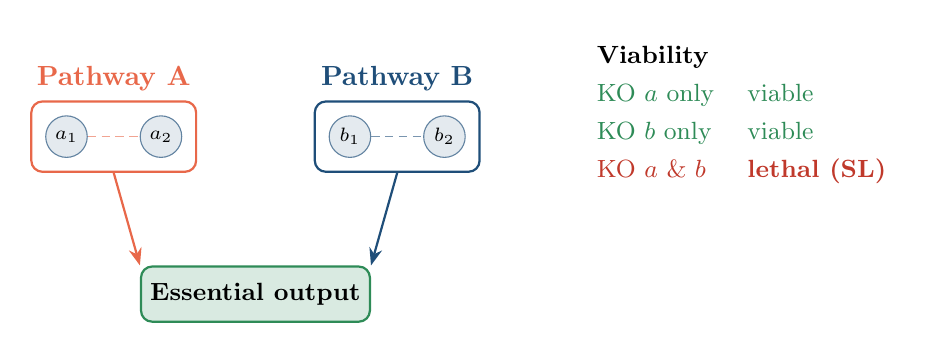
\begin{tikzpicture}[
  gene/.style={circle,draw=sriblue!70,fill=sriblue!12,minimum size=15pt,inner sep=0pt,font=\scriptsize},
  proc/.style={rounded corners,draw=srigray,thick,inner sep=8pt},
  lab/.style={font=\small\bfseries},
  >={Stealth[length=2.2mm]}]

  % Essential process node
  \node[rectangle,rounded corners,fill=srigreen!18,draw=srigreen,thick,minimum width=2.4cm,minimum height=0.7cm] (E) at (0,0) {\small\bfseries Essential output};

  % Pathway A
  \node[gene] (a1) at (-2.4,2.0) {$a_1$};
  \node[gene] (a2) at (-1.2,2.0) {$a_2$};
  \node[draw=sriaccent,thick,rounded corners,fit=(a1)(a2),inner sep=5pt,label=above:{\color{sriaccent}\bfseries Pathway A}] (A) {};

  % Pathway B
  \node[gene] (b1) at (1.2,2.0) {$b_1$};
  \node[gene] (b2) at (2.4,2.0) {$b_2$};
  \node[draw=sriblue,thick,rounded corners,fit=(b1)(b2),inner sep=5pt,label=above:{\color{sriblue}\bfseries Pathway B}] (B) {};

  \draw[->,sriaccent,thick] (A.south) -- (E.north west);
  \draw[->,sriblue,thick]   (B.south) -- (E.north east);
  \draw[densely dashed,sriaccent!60] (a1)--(a2);
  \draw[densely dashed,sriblue!60] (b1)--(b2);

  % viability table
  \node[anchor=west] at (4.0,2.3) {\small\begin{tabular}{ll}
    \multicolumn{2}{l}{\bfseries Viability}\\
    \color{srigreen}KO $a$ only & \color{srigreen}viable\\
    \color{srigreen}KO $b$ only & \color{srigreen}viable\\
    \color{srired}KO $a$ \& $b$ & \color{srired}\bfseries lethal (SL)\\
  \end{tabular}};

\end{tikzpicture}
\caption{The topological basis of synthetic lethality. Two redundant pathways
($A$,$B$) independently sustain an essential output. Removing one is buffered by
the other; removing both is lethal. A gene in $A$ and a gene in $B$ are
synthetic-lethal --- a fact about their \emph{network positions}, invisible to a
model that sees only per-gene features.}
\label{fig:mechanism}
\end{figure}

% ===========================================================================
\section{Research Questions \& Hypotheses}

\begin{description}[leftmargin=1.6em,style=nextline]
\item[RQ1] Does encoding the gene-interaction graph let a GNN predict SL better
than strong non-graph baselines (XGBoost, MLP, KGE)?
\item[RQ2] Does the GNN advantage persist for \emph{cold genes} absent from
training, where memorization-based baselines cannot generalize?
\item[RQ3] Is the GNN advantage \emph{causally} attributable to topology, or to
confounds (node features, degree popularity)?
\end{description}

\begin{hypobox}{Hypotheses}
\textbf{H1.} Transductively, GNN $\approx$ random-walk embeddings $\gg$ MLP/XGBoost.\\
\textbf{H2.} Inductively (cold-gene), GNN $\gg$ all baselines, which fall to chance.\\
\textbf{H3.} Destroying topology (rewire/empty graph) collapses the GNN to the
feature-only baseline, proving the advantage is structural.
\end{hypobox}

% ===========================================================================
\section{Data}

\begin{table}[h]
\centering
\small
\begin{tabular}{>{\raggedright\arraybackslash}p{0.24\linewidth} >{\raggedright\arraybackslash}p{0.40\linewidth} >{\raggedright\arraybackslash}p{0.28\linewidth}}
\toprule
\rowcolor{sriblue}\color{white}\textbf{Resource} & \color{white}\textbf{Content} & \color{white}\textbf{Role}\\
\midrule
\rowcolor{srirow} SynLethDB 2.0 (via KG4SL) & $\sim$73k human SL gene pairs & Positive labels\\
KG4SL knowledge graph & $\sim$476k gene--gene edges (interaction, regulation, co-expression relations) & Message-passing graph\\
\rowcolor{srirow} Explicit non-SL pairs & $\sim$3k experimentally non-lethal pairs & Hard negatives (seed)\\
Degree-matched samples & Negatives drawn to match positive degree distribution & Shortcut-free negatives\\
\bottomrule
\end{tabular}
\caption{All data are public and de-identified. The SL/non-SL relations are
removed from the message-passing graph to prevent leakage.}
\label{tab:data}
\end{table}

\noindent\textbf{Controlled synthetic benchmark.} In parallel I will build a
generator in which SL is \emph{defined} by topology (genes in different
redundant modules of the same essential process), with deliberately
uninformative node features. Because the only signal is structural, this
isolates the GNN's contribution and powers the falsification ablation.

% ===========================================================================
\section{Methods}

\subsection{Model (ours): inductive heterogeneous GNN}
A GraphSAGE encoder produces a gene embedding by aggregating its neighborhood
over $L{=}3$ message-passing layers:
\begin{equation}
h_v^{(l)} = \sigma\!\Big( W^{(l)} \big[\, h_v^{(l-1)} \,\big\Vert\,
\textstyle\operatorname*{AGG}_{u\in\mathcal{N}(v)} h_u^{(l-1)} \,\big] \Big),
\qquad z_v = h_v^{(L)} .
\label{eq:sage}
\end{equation}
Because Eq.~\eqref{eq:sage} reads only the local neighborhood (not a per-node
lookup table), embeddings transfer to genes unseen in training --- the property
that enables cold-gene prediction. A \emph{symmetric} decoder scores a pair
(SL is undirected):
\begin{equation}
\hat{s}_{ij} = \operatorname{sigmoid}\!\Big(\operatorname{MLP}\big[\,
z_i + z_j \,\big\Vert\, |z_i - z_j| \,\big]\Big).
\label{eq:decoder}
\end{equation}
Training minimizes binary cross-entropy over positives $\mathcal{P}$ and
sampled negatives $\mathcal{N}$:
\begin{equation}
\mathcal{L} = -\!\!\sum_{(i,j)\in\mathcal{P}}\!\!\log \hat{s}_{ij}
              -\!\!\sum_{(i,j)\in\mathcal{N}}\!\!\log\big(1-\hat{s}_{ij}\big).
\label{eq:bce}
\end{equation}

\subsection{Baselines (fair, shared trainer)}
\begin{table}[h]
\centering
\small
\begin{tabular}{>{\raggedright\arraybackslash}p{0.20\linewidth} >{\raggedright\arraybackslash}p{0.30\linewidth} >{\raggedright\arraybackslash}p{0.42\linewidth}}
\toprule
\rowcolor{sriblue}\color{white}\textbf{Model} & \color{white}\textbf{Uses graph?} & \color{white}\textbf{What it tests}\\
\midrule
\rowcolor{srirow} \textbf{GNN (ours)} & yes (message passing) & topology-aware inductive prediction\\
XGBoost & no & strong tabular baseline on pair features\\
\rowcolor{srirow} MLP & no (features only) & structure-blind control\\
node2vec + decoder & structure via memorized walks & transductive-only structure\\
\rowcolor{srirow} TransE / DistMult (KGE) & structure via memorized embeddings & shallow KG baselines\\
\bottomrule
\end{tabular}
\caption{The MLP and XGBoost share the pair-feature construction; node2vec/KGE
share the decoder. Any gap reflects the value of message passing alone.}
\label{tab:models}
\end{table}

\subsection{Leakage-safe splits}
\begin{itemize}[leftmargin=1.4em,itemsep=1pt]
\item \textbf{Transductive:} pairs split randomly; all genes seen in training.
\item \textbf{Inductive (cold-gene):} whole \emph{genes} held out; test pairs
touch unseen genes, which are removed from the training message-passing graph
and only reattached at evaluation. This is the leakage-safe ``group split''
analogue and the decisive test of generalization.
\end{itemize}

\subsection{Degree-matched negatives (removing the shortcut)}
With uniform-random negatives, SL genes (well-studied hubs) have higher degree
than random genes, so a single degree feature separates classes --- a confound
that lets a feature model appear competitive. I instead sample negatives whose
endpoint degrees match the positives:
\[
\Pr\big[(i',j')\in\mathcal{N}\big] \;\propto\;
\mathbb{1}\!\left[\,b(i')=b(i)\,\wedge\,b(j')=b(j)\,\right],
\]
where $b(\cdot)$ is a node's degree-quantile bin and $(i,j)$ is a template
positive. This forces reliance on \emph{which} genes interact, not \emph{how
connected} they are.

\subsection{Metrics (imbalance-aware)}
Area under the precision--recall curve (AUPRC) as the primary metric, plus
AUROC, and ranking metrics that mirror wet-lab triage of a candidate shortlist:
\begin{equation}
\mathrm{Hits}@K = \frac{1}{|\mathcal{P}|}\sum_{p\in\mathcal{P}}
\mathbb{1}[\operatorname{rank}(p)\le K],
\qquad
\mathrm{MRR} = \frac{1}{|\mathcal{P}|}\sum_{p\in\mathcal{P}}
\frac{1}{\operatorname{rank}(p)} .
\label{eq:rank}
\end{equation}
All results are reported as mean\,$\pm$\,std over 5 seeds.

% ===========================================================================
\section{Model Pipeline}

Figure~\ref{fig:pipeline} contrasts the two information pathways under test: the
GNN consumes the interaction graph, whereas the feature baselines (XGBoost, MLP)
never see an edge. Because every model shares the same decoder and training
loop, any performance gap is attributable to message passing alone.

\begin{figure}[h]
\centering
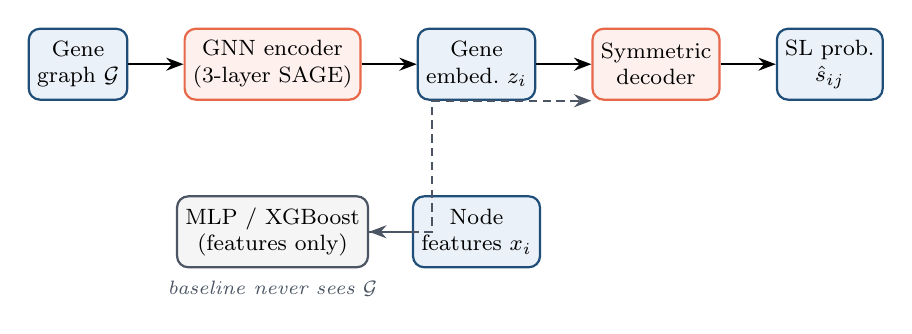
\begin{tikzpicture}[
  node distance=6mm and 7mm,
  box/.style={rounded corners,draw=sriblue,fill=srilight,thick,minimum height=0.9cm,align=center,font=\footnotesize,inner sep=3pt},
  red/.style={rounded corners,draw=sriaccent,fill=sriaccent!10,thick,minimum height=0.9cm,align=center,font=\footnotesize,inner sep=3pt},
  gray/.style={rounded corners,draw=srigray,fill=gray!8,thick,minimum height=0.9cm,align=center,font=\footnotesize,inner sep=3pt},
  >={Stealth[length=2.2mm]}]

  \node[box] (g) {Gene\\graph $\mathcal{G}$};
  \node[red,right=of g] (enc) {GNN encoder\\(3-layer SAGE)};
  \node[box,right=of enc] (z) {Gene\\embed.\ $z_i$};
  \node[red,right=of z] (dec) {Symmetric\\decoder};
  \node[box,right=of dec] (s) {SL prob.\\$\hat{s}_{ij}$};

  \draw[->,thick] (g)--(enc);
  \draw[->,thick] (enc)--(z);
  \draw[->,thick] (z)--(dec);
  \draw[->,thick] (dec)--(s);

  % baseline branch (ignores edges)
  \node[gray,below=12mm of enc] (mlp) {MLP / XGBoost\\(features only)};
  \node[box,below=12mm of z] (xf) {Node\\features $x_i$};
  \draw[->,thick,densely dashed,srigray] (xf)--(mlp);
  \draw[->,thick,densely dashed,srigray] (mlp.east) -- ++(0.8,0) |- (dec.south west);
  \node[srigray,font=\scriptsize\itshape,below=1pt of mlp] {baseline never sees $\mathcal{G}$};

\end{tikzpicture}
\caption{The GNN (orange) propagates over $\mathcal{G}$; the feature baselines
(gray) bypass the graph entirely. The comparison isolates the contribution of
message passing.}
\label{fig:pipeline}
\end{figure}

% ===========================================================================
\section{Ablations \& Interpretability}

\subsection{Falsification: topology-removal ablation}
The headline experiment trains the \emph{identical} GNN on three graphs and
compares against the structure-blind MLP:
\begin{table}[h]
\centering
\small
\begin{tabular}{>{\raggedright\arraybackslash}p{0.22\linewidth} >{\raggedright\arraybackslash}p{0.50\linewidth} >{\raggedright\arraybackslash}p{0.20\linewidth}}
\toprule
\rowcolor{sriblue}\color{white}\textbf{Condition} & \color{white}\textbf{Graph given to the GNN} & \color{white}\textbf{Expected}\\
\midrule
\rowcolor{srirow} Intact & true interaction graph & high\\
Rewired & random graph, same node/edge count & $\approx$ chance\\
\rowcolor{srirow} Empty & no edges (GNN $\to$ MLP) & $\approx$ chance\\
\bottomrule
\end{tabular}
\caption{If the GNN's advantage is real, destroying structure must erase it.}
\label{tab:ablation}
\end{table}

\noindent Additional ablations: per-relation removal (which interaction type
matters), message-passing depth ($1$--$4$ layers), and negative-sampling
strategy (random vs.\ degree-matched).

\subsection{Interpretability that yields a discovery}
Using GNNExplainer/attention, I will extract the small subgraph most
responsible for each high-confidence SL prediction and verify it corresponds to
a parallel-pathway motif. As a concrete validation I will check recovery of
\textbf{known \textit{KRAS} synthetic-lethal partners}, then produce a ranked
shortlist of \emph{novel} candidate SL partners, each accompanied by an
interpretable pathway-redundancy explanation.

% ===========================================================================
\section{Expected Outcomes \& Success Criteria}

This is a proposal; the table states \emph{targets and qualitative
expectations}, not measured results.

\begin{table}[h]
\centering
\small
\begin{tabular}{>{\raggedright\arraybackslash}p{0.26\linewidth} >{\raggedright\arraybackslash}p{0.66\linewidth}}
\toprule
\rowcolor{sriblue}\color{white}\textbf{Regime / artifact} & \color{white}\textbf{Expected pattern (success criterion)}\\
\midrule
\rowcolor{srirow} Transductive & GNN $\approx$ node2vec $\gg$ XGBoost/MLP: structure carries the signal.\\
Inductive (cold-gene) & GNN $\gg$ all baselines, which approach chance: only the GNN generalizes structurally.\\
\rowcolor{srirow} Topology ablation & Intact $\gg$ rewired $\approx$ empty $\approx$ MLP: the advantage is causal.\\
Interpretability & Recover known \textit{KRAS} SL partners; deliver a ranked novel shortlist.\\
\rowcolor{srirow} Honesty clause & A null result (GNN $\approx$ baselines) will be reported as-is; the task is constructed so a correct GNN \emph{can} win.\\
\bottomrule
\end{tabular}
\caption{Success is defined by the \emph{pattern} across regimes, not a single
headline number.}
\label{tab:success}
\end{table}

% ===========================================================================
\section{Eight-Week Timeline}

\begin{table}[h]
\centering
\small
\begin{tabular}{>{\raggedright\arraybackslash}p{0.14\linewidth} >{\raggedright\arraybackslash}p{0.78\linewidth}}
\toprule
\rowcolor{sriblue}\color{white}\textbf{Weeks} & \color{white}\textbf{Milestones}\\
\midrule
\rowcolor{srirow} 1--2 & Data pipeline (KG4SL download, leakage-free graph, degree-matched negatives); synthetic generator.\\
3--4 & Models in PyG: GNN encoder/decoder; baselines XGBoost, MLP, node2vec, KGE; shared trainer.\\
\rowcolor{srirow} 5 & Transductive + inductive experiments, 5 seeds, imbalance-aware metrics.\\
6 & Ablations: topology removal, relation type, depth, negatives.\\
\rowcolor{srirow} 7 & Interpretability + \textit{KRAS} case study; candidate shortlist.\\
8 & Figures, tables, manuscript; reproducibility package.\\
\bottomrule
\end{tabular}
\caption{Schedule for the eight-week SRI cohort.}
\label{tab:timeline}
\end{table}

% ===========================================================================
\section{Reproducibility, Tooling, and Ethics}

Implementation uses \textbf{PyTorch Geometric}, the leading GNN library
(heterogeneous graphs, link-prediction utilities, neighbor sampling for scale).
All code, configs, seeds, and a data manifest (accession, version, license,
date) will be released. No human subjects are involved; all inputs are public
and de-identified. Predictions are research-only and hypothesis-generating, to
be confirmed by wet-lab follow-up; no clinical claims are made.

% ===========================================================================
\section*{Selected References}
\small
\begin{enumerate}[leftmargin=1.4em,itemsep=0pt]
\item Hamilton, Ying, Leskovec. \textit{Inductive Representation Learning on
Large Graphs (GraphSAGE)}. NeurIPS, 2017.
\item Wang et al. \textit{SynLethDB 2.0: a web-based knowledge graph database on
synthetic lethality}. Database, 2022.
\item Zheng et al. \textit{KG4SL: knowledge graph neural network for synthetic
lethality prediction in human cancers}. Bioinformatics, 2021.
\item O'Neil, Haber, Buckanovich. \textit{Synthetic lethality and cancer}.
Nature Reviews Genetics, 2017.
\item Ying et al. \textit{GNNExplainer: Generating Explanations for Graph Neural
Networks}. NeurIPS, 2019.
\end{enumerate}

\end{document}
